\chapter{Genetic Algorithms}
\label{ch:ga}

\chapterguide%
  {Know local search from \chapref{ch:localsearch}, be comfortable with NumPy arrays and random numbers, and know what a regression model and its RMSE are.}
  {name the parts of a genetic algorithm and what each contributes; encode a real-valued problem as a chromosome; implement tournament selection, blend crossover, Gaussian mutation and elitism; evaluate a stochastic optimiser over repeated seeds; and decide when an evolutionary method is justified against an exact one.}

Every search in \chapref{ch:localsearch} changes one candidate at a time: one queen on one board, one word added to one sentence. Each option only ever grows by itself. But two half-good solutions often have complementary strengths. What if they could combine?

Nature does this all the time, with two parents and a child that gets a bit of each. A \term{genetic algorithm} (GA) applies the same idea to candidate solutions. It improves a whole population through selection, recombination and random mutation, and it needs only a scoring function, not derivatives or convexity. Lab~8 tests a GA on a known one-dimensional function, then fits linear-regression coefficients. Ordinary least squares provides an exact, faster reference, so the aim is to evaluate a stochastic optimiser, not to claim it beats an exact method.

\section{Breeding boards: the idea on eight queens}

Start with the puzzle from \chapref{ch:localsearch}. A GA keeps a population of boards, say 50 random ones, and writes each board as eight digits, one per column, each saying which row that column's queen is in. Each board gets a \term{fitness}: the fewer attacking pairs, the fitter it is.

\begin{analogy}
Think of a raffle for the right to breed. Eight queens make 28 pairs, and a board gets one ticket for every pair that does \emph{not} attack. A board with 3 attacking pairs holds 25 tickets, and one with 10 holds 18. Draw two tickets to choose two parents. Fitter boards are likelier to be drawn, but even a poor board has a chance, which keeps variety in the population.
\end{analogy}

Two more steps make a child. In \term{crossover} we cut both parents at a random column and join the pieces. In \term{mutation}, now and then, one queen in the child jumps to a random row, which can create a row neither parent had (\figref{fig:breeding}).

\begin{utpfig}[Crossover and mutation on eight-queens boards]{A lucky pairing, chosen to show both operators. Each digit gives the row of one column's queen. Crossover cuts both parents after the same column and joins the left of one to the right of the other, and the child has only one attacking pair. Mutation then changes one digit to a row neither parent had in that column, and this board is solved.}{fig:breeding}
\begin{tikzpicture}[font=\small,
  ga/.style={cell,minimum width=0.58cm,minimum height=0.6cm,font=\small\bfseries\color{UTPNavy}},
  gb/.style={cellalt,minimum width=0.58cm,minimum height=0.6cm,font=\small\bfseries\color{UTPNavy}},
  gm/.style={cellbad,minimum width=0.58cm,minimum height=0.6cm,font=\small\bfseries\color{UTPRed}}]
\def\s{0.6}
\node[tagb,anchor=south west] at (-0.3,1.42) {parent 1: 5 attacking pairs};
\node[tagb,anchor=north west] at (-0.3,-0.22) {parent 2: 6 attacking pairs};
\foreach \d [count=\i from 0] in {1,4,6,3,1,6,2,5}{\node[ga] at (\s*\i,1.1) {\d};}
\foreach \d [count=\i from 0] in {1,4,2,2,0,7,4,2}{\node[gb] at (\s*\i,0.1) {\d};}
\draw[draw=UTPRed,dashed,thick] (\s*3+\s/2,1.42) -- (\s*3+\s/2,-0.22);
\node[utplabel,anchor=west,color=UTPRed] at (\s*3+\s/2+0.05,0.6) {cut};
\draw[utparrow] (4.7,0.6) -- (6.0,0.6) node[midway,above,utplabel] {crossover};
\begin{scope}[xshift=6.45cm]
\node[tagb,anchor=south] at (\s*3.5,0.92) {child: 1 attacking pair};
\foreach \d [count=\i from 0] in {1,4,6,3}{\node[ga] at (\s*\i,0.6) {\d};}
\foreach \d [count=\i from 4] in {0,7,4,2}{\node[gb] at (\s*\i,0.6) {\d};}
\end{scope}
\begin{scope}[xshift=6.45cm,yshift=-0.75cm]
\foreach \d [count=\i from 0] in {1,4,6,3}{\node[ga] at (\s*\i,0) {\d};}
\foreach \d [count=\i from 4] in {0,7}{\node[gb] at (\s*\i,0) {\d};}
\node[gm] at (\s*6,0) {5};
\node[gb] at (\s*7,0) {2};
\node[tagb,anchor=north] at (\s*3.5,-0.34) {after mutation: no attacks, solved};
\draw[utpptr,draw=UTPRed] (\s*6,0.98) -- (\s*6,0.34);
\node[utplabel,anchor=west,color=UTPRed] at (\s*7+0.42,0.68) {mutate $4\to5$};
\end{scope}
\end{tikzpicture}
\end{utpfig}

Repeat this to fill a new generation and let the children replace the population. Good pieces from two parents can then meet in one child, in a single step that a hill climber could not take. Here is that loop in Python, as the demo runs it:

\lstinputlisting[style=utppython,firstline=79,lastline=98]{all_experiments/demo_local_search.py}

Now the honest part. How well does it work on eight queens? In the demo, 171 of 200 runs find a solution within 1,000 generations, with a median of 328 generations among those that succeed. The work comes to about 27,000 boards per puzzle solved. Simulated annealing needed about 1,100.

\begin{keyidea}
Breeding boards sounds like the coolest idea in this book, and on eight queens the dumbest-sounding idea, annealing, does the job with less than a tenth of the work. When an idea sounds exciting, race it against a simple one first.
\end{keyidea}

GAs still earn their keep elsewhere. NASA used an evolutionary algorithm, a cousin of this one, to design an antenna for its Space Technology 5 mission. The result looks like a bent paper clip, nothing a human designer would draw, and it flew in space in 2006. Lab~8 tests the method on a problem where we know the exact answer, which is the fairest test of all.

\section{Vocabulary}

\begin{utptable}
\begin{tabularx}{\linewidth}{@{}>{\bfseries\leavevmode\color{UTPNavy}}m{0.14\linewidth}m{0.34\linewidth}m{0.21\linewidth}X@{}}
\toprule
\rowcolor{UTPPaleBlue!92}
\utpth{Term} & \utpth{Meaning} & \utpth{On eight queens} & \utpth{In Lab~8} \\
\midrule
Chromosome & One candidate solution, as a vector of genes & Eight digits, one per column & Five real numbers: intercept plus four coefficients \\
Gene & One component of a chromosome & One queen's row & One coefficient \\
Population & The set of chromosomes alive in one generation & 50 boards & 100 (or 40 in the sensitivity study) \\
Fitness & The score to be optimised & Pairs not attacking; higher is better & Training mean squared error; lower is better \\
Selection & Choosing parents, biased towards good fitness & Tickets (roulette wheel) & Tournament of three \\
Crossover & Combining two parents into children & Cut and join & Blend crossover \\
Mutation & Random perturbation of a child & One queen jumps & Gaussian noise on a random subset of genes \\
Elitism & Copying the best chromosomes unchanged into the next generation & None & The best 4 (or 2) survive \\
Generation & One pass of evaluate, select, cross, mutate, replace & Up to 1,000 passes & 160 passes per run \\
\bottomrule
\end{tabularx}
\end{utptable}

\section{One generation}

\figref{fig:ga-loop} combines selection pressure, recombination, mutation and preservation of the best candidates.

\begin{utpfig}[The genetic algorithm loop]{Selection favours better solutions, crossover recombines parents, mutation introduces variation, and elitism preserves the best candidates.}{fig:ga-loop}
\begin{tikzpicture}[
  b/.style={draw=UTPBlue,fill=UTPPaleBlue,rounded corners=2mm,minimum width=2.4cm,minimum height=0.9cm,align=center,font=\scriptsize\color{UTPNavy}},
  arr/.style={-{Stealth[length=2mm]},thick,draw=UTPTeal}
]
\node[b] (p) {Population};
\node[b,right=0.35cm of p] (fit) {Evaluate\\fitness};
\node[b,right=0.35cm of fit] (sel) {Select\\parents};
\node[b,right=0.35cm of sel] (cross) {Crossover};
\node[b,right=0.35cm of cross] (mut) {Mutation};
\node[b,below=1.0cm of sel,fill=UTPPaleTeal,draw=UTPGreen] (rep) {New generation\\= elites + children};
\draw[arr] (p)--(fit); \draw[arr] (fit)--(sel); \draw[arr] (sel)--(cross); \draw[arr] (cross)--(mut);
\draw[arr] (mut.south) |- (rep.east);
\draw[arr] (rep.west) -| (p.south);
\draw[arr,draw=UTPGreen,dashed] (fit.south) -- ++(0,-0.55) -| (rep.north) node[pos=0.25,below,xshift=-1cm,utplabel,color=UTPGreen] {best few copied unchanged (elitism)};
\end{tikzpicture}
\end{utpfig}

The lab uses the same loop for a single number $x$ and for a five-gene vector. The single-number version, which minimises $(x-3)^2$, shows all the moving parts in a few lines:

\lstinputlisting[style=utppython,firstline=28,lastline=39]{all_experiments/lab08_genetic_algorithm_regression_worked.py}

Vectorised operators avoid looping over individuals, so 160 generations of 100 chromosomes take a few hundredths of a second.

\section{Encoding: the chromosome is the answer}

For $\hat y=p_0+p_1x_1+\dots+p_4x_4$, encode each chromosome as five real coefficients. The GA searches the same space as least squares, which is what makes a direct comparison possible. Two details matter:

\begin{description}
  \item[Initialisation matters.] Charges are in thousands of dollars. Draw coefficients with mean~0 and standard deviation~5000, then shift the intercept towards the mean charge. Starting from $\mathcal N(0,1)$ would place the whole population far from useful values.
  \item[Standardise the inputs.] Age (18--64) and smoker status (0--1) have very different scales. Standardise all four predictors using training statistics so that a mutation step means roughly the same thing for each coefficient.
\end{description}

\begin{intuition}
The chromosome \emph{is} the candidate answer, read by the fitness function. Operators depend on the encoding: blend crossover suits real coefficients, cut-and-join suits eight-queens boards, and neither would make sense on a route that must visit every city exactly once.
\end{intuition}

\section{The operators}

\subsection{Fitness}

Fitness is training mean squared error. The lab evaluates it for the whole population in one matrix product:

\lstinputlisting[style=utppython,firstline=66,lastline=68]{all_experiments/lab08_genetic_algorithm_regression_worked.py}

Evaluating 100 five-gene chromosomes on 1,070 training rows produces a $100\times1{,}070$ prediction matrix, computed in one step rather than in a Python loop.

\subsection{Selection}

\term{Tournament selection} samples $k$ chromosomes and keeps the fittest, like picking the winner of a small heat; Lab~8 uses $k=3$. Unlike \term{roulette-wheel} selection (\figref{fig:roulette}), which is the raffle from eight queens, it does not depend on the scale of the fitness values and needs no conversion when lower is better. The tournament size sets the selection pressure. With $k=1$ there is no selection at all, and on Lab~8 the seed-to-seed spread jumps from $0.002$ to about 11.5.

\begin{utpfig}[Roulette-wheel selection]{Arc widths are proportional to fitness: B is selected four times as often as D. Tournament selection favours fitter candidates without depending on fitness scale.}{fig:roulette}
\begin{tikzpicture}[font=\small]
\node[utplabel,font=\small\bfseries\color{UTPNavy}] at (0,2.1) {Selection probabilities};
\def\rad{1.75}
\foreach \a/\b/\lbl/\col in {0/144/B/UTPBlue, 144/252/A/UTPTeal, 252/324/C/UTPOrange, 324/360/D/UTPRed}{
  \fill[\col!28,draw=\col,thick] (0,0) -- (\a:\rad) arc[start angle=\a,end angle=\b,radius=\rad] -- cycle;
  \pgfmathsetmacro{\mid}{(\a+\b)/2}
  \node[font=\small\bfseries\color{UTPNavy}] at (\mid:0.65*\rad) {\lbl};
}
\node[utplabel,anchor=north,align=center] at (0,-2.0)
  {Fitness $(B,A,C,D)=(4,3,2,1)$};
\begin{scope}[xshift=4.0cm,yshift=-0.4cm]
\def\L{7.2}
\node[utplabel,font=\small\bfseries\color{UTPNavy}] at (0.5*\L,2.5)
  {Cumulative probability};
\foreach \s/\e/\lbl/\col in {0/0.40/B/UTPBlue, 0.40/0.70/A/UTPTeal, 0.70/0.90/C/UTPOrange, 0.90/1.0/D/UTPRed}{
  \pgfmathsetmacro{\x}{\s*\L}
  \pgfmathsetmacro{\w}{(\e-\s)*\L}
  \fill[\col!28,draw=\col,thick] (\x,0) rectangle ++(\w,0.85);
  \node[font=\small\bfseries\color{UTPNavy}] at (\x+\w/2,0.42) {\lbl};
}
\foreach \v/\x in {0/0, 0.40/0.40, 0.70/0.70, 0.90/0.90, 1.0/1.0}{
  \pgfmathsetmacro{\xx}{\x*\L}
  \node[utplabel] at (\xx,-0.28) {\v};
}
\draw[-{Stealth[length=2.4mm]},line width=1.2pt,draw=UTPNavy] (0.54*\L,1.5) -- (0.54*\L,0.95);
\node[utplabel,anchor=south,color=UTPNavy] at (0.54*\L,1.55) {\texttt{rand} $=0.54\ \Rightarrow$ pick A};
\node[utplabel,anchor=north,align=center,text width=6.8cm] at (0.5*\L,-0.75)
  {The draw $0.54$ falls in A\textquotesingle s interval, $0.40$ to $0.70$.};
\end{scope}
\end{tikzpicture}
\end{utpfig}

\subsection{Crossover and mutation}

Cutting a list of real coefficients and joining the pieces would work poorly, because a good value of one gene is not tied to a position. \term{Blend crossover} forms $\alpha\,a+(1-\alpha)\,b$ from two parents instead. With $\alpha\in[0,1]$, children lie between them. The regression GA uses $\alpha\in[-0.1,1.1]$, which allows a child to land just beyond a parent (\figref{fig:crossover}). \term{Gaussian mutation} adds noise to a random 15\,\% of genes using per-gene step sizes. Without it the population can only contract: with the mutation rate set to zero, Lab~8's median test RMSE stays stuck at about 6,534 instead of reaching 5,829.

\begin{utpfig}[Crossover and mutation for real-valued genes]{Left: blend crossover places children between parents or slightly beyond them. Right: Gaussian mutation perturbs a child by a random step.}{fig:crossover}
\begin{tikzpicture}[font=\small]
\begin{scope}
\node[font=\bfseries\color{UTPNavy}] at (2.0,2.65) {Blend crossover};
\draw[-{Stealth[length=2mm]},draw=UTPMuted] (-0.2,0)--(4.4,0) node[right,font=\scriptsize] {$p_1$};
\draw[-{Stealth[length=2mm]},draw=UTPMuted] (0,-0.2)--(0,1.85) node[above,font=\scriptsize] {$p_2$};
\node[circle,fill=UTPBlue,inner sep=2.2pt,label={[utplabel,color=UTPBlue]above:parent $a$}] (P1) at (0.7,1.35) {};
\node[circle,fill=UTPTeal,inner sep=2.2pt,label={[utplabel,color=UTPTeal]below:parent $b$}] (P2) at (3.6,0.45) {};
\draw[draw=UTPMuted!60,dashed] (P1)--(P2);
\node[circle,fill=UTPOrange,inner sep=2.2pt] (Ch) at (1.86,1.0) {};
\node[utplabel,anchor=west,color=UTPOrange] at (2.0,1.28) {child, $\alpha=0.6$};
\node[utplabel,anchor=north,align=center,text width=4.8cm] at (2.0,-1.15)
  {$\alpha\in[-0.1,1.1]$ lets a child land just beyond a parent};
\end{scope}
\begin{scope}[xshift=6.6cm]
\node[font=\bfseries\color{UTPNavy}] at (2.2,2.65) {Gaussian mutation};
\draw[-{Stealth[length=2mm]},draw=UTPMuted] (-0.2,0)--(4.4,0) node[right,font=\scriptsize] {$p_1$};
\draw[-{Stealth[length=2mm]},draw=UTPMuted] (0,-0.2)--(0,1.85) node[above,font=\scriptsize] {$p_2$};
\node[circle,fill=UTPOrange,inner sep=2.2pt,label={[utplabel,color=UTPOrange]below:child}] (C) at (1.9,0.9) {};
\draw[draw=UTPOrange!35,fill=UTPOrange!10] (1.9,0.9) circle (0.75);
\node[circle,fill=UTPRed,inner sep=2.2pt,label={[utplabel,color=UTPRed]above right:mutated child}] (M) at (2.45,1.3) {};
\draw[utpptr,draw=UTPRed] (C)--(M);
\node[utplabel,anchor=north,align=center,text width=5.2cm] at (2.2,-1.15)
  {each gene moves by $\mathcal N(0,\sigma)$ with probability $0.15$; $\sigma$ is set per gene};
\end{scope}
\end{tikzpicture}
\end{utpfig}

\subsection{Elitism}

\term{Elitism} copies the best chromosomes unchanged into the next generation, so that selection or mutation cannot lose them. Think of an athletics squad that always keeps its current record holder. It costs a few population slots and means that the best fitness in the population can never get worse. Without elites, the best member of the population got worse in 54 of 159 generations on one Lab~8 run.

\begin{keyidea}
Selection favours good candidates, crossover recombines, mutation explores and elitism preserves. Tournament size~3, 15\,\% mutation and four elites are one workable balance, not universal settings.
\end{keyidea}

\section{Verifying before trusting}

Wrong fitness signs or mutation scales may not raise any error message: the code just runs and gives poor answers. So Lab~8 first minimises $f(x)=(x-3)^2$, whose answer we know, reaching about $10^{-5}$ from $x=3$ in 80 generations. Only then does it move on to regression, where least squares supplies a second check.

\section{Judging a stochastic optimiser}

A GA uses random numbers, so one seed shows only one outcome. Lab~8 reports results over ten seeds and compares them with an exact method.

\begin{utptable}
\begin{tabularx}{\linewidth}{@{}>{\bfseries\leavevmode\color{UTPNavy}}m{0.28\linewidth}>{\centering\arraybackslash}X>{\centering\arraybackslash}X>{\centering\arraybackslash}X@{}}
\toprule
\rowcolor{UTPPaleBlue!92}
\utpth{Method} & \utpth{Median test RMSE} & \utpth{SD across seeds} & \utpth{Median runtime} \\
\midrule
GA, population 100 & 5829.38 & 0.002 & 0.04 s \\
GA, population 40 & 5829.38 & 0.026 & 0.02 s \\
Ordinary least squares & 5829.38 & --- & $<$ 0.001 s \\
\bottomrule
\end{tabularx}
\end{utptable}

Three lessons follow:

\begin{description}
  \item[The GA approaches the optimum.] Runs agree within a few thousandths and match OLS performance, and the median coefficients match OLS to one decimal place.
  \item[It did not beat the optimum.] Least squares solves the same problem exactly and faster. Agreement verifies the GA; it shows no advantage over OLS.
  \item[Population size trades speed for spread.] Forty chromosomes halve the runtime with the same median, but increase seed-to-seed standard deviation by an order of magnitude. Judge that trade against the cost of a poor run.
\end{description}

\begin{pitfall}
Report the median and spread across independent seeds, not one run or the best run presented as typical. A lucky seed says nothing about the next one. On eight queens the median successful run took 328 generations, and 29 of the 200 runs did not finish at all.
\end{pitfall}

\section{When is a genetic algorithm the right tool?}

Least squares suits Lab~8's smooth, convex, unconstrained objective. Recall the bowl from \chapref{ch:fuzzy}: one lowest point and a formula that jumps straight there. Consider a GA when the problem is nothing like a bowl:

\begin{itemize}
  \item the objective is \textbf{non-differentiable} or only available as a black box (a simulation, a physical test rig);
  \item some variables are \textbf{discrete or mixed} (which features to include, which route to take, which schedule to run), so there is no gradient to follow;
  \item the objective is \textbf{multimodal}, with many local optima that trap gradient methods;
  \item the constraints are \textbf{awkward}: business rules, integer budgets, or feasibility checks that are easy to test and impossible to write as equations.
\end{itemize}

Integer coefficients, penalties on non-zero coefficients or a plateaued loss would invalidate ordinary least squares. A GA would need a revised fitness function and possibly new operators, and the deliverable asks you to identify one such change.

\begin{chapterrecap}
\begin{itemize}
  \item A GA evolves a population: fitter candidates are selected, recombined and mutated, and the best may be kept unchanged.
  \item The encoding decides the operators. Eight digits suit cut-and-join; real coefficients suit blending and Gaussian noise.
  \item Verify on a problem with a known answer, then report the median and spread over independent seeds.
  \item A GA that matches an exact method has been verified, not vindicated. Race it against something simple, and reach for it when the problem has no formula and no gradient.
\end{itemize}
\end{chapterrecap}

\begin{quickcheck}
\begin{enumerate}
  \item What is the chromosome in Lab~8, and how many genes does it have?
  \item Why does the lab standardise the predictors before running the GA, when least squares would give the same fit either way?
  \item What can happen to the best fitness in the population without elitism, and why?
  \item Blend crossover with $\alpha\in[0,1]$ can only produce children between the parents. What does that do to a population over many generations, and which two choices in the lab counteract it?
  \item Ten seeds gave test RMSE within $0.002$ of each other. Why is that a stronger statement than one run that hit the OLS value exactly?
  \item On eight queens, a board has 4 attacking pairs. How many raffle tickets does it hold?
\end{enumerate}
\end{quickcheck}

\begin{checkanswers}
\begin{enumerate}
  \item A vector of five real numbers: the intercept and the coefficients of age, BMI, children and smoker status.
  \item One mutation step size is used for every coefficient gene. With unstandardised inputs the same step would be huge for one coefficient and negligible for another; least squares is indifferent because it solves the problem exactly rather than searching it.
  \item It can get worse: the best chromosome might not be selected, or might be crossed or mutated away, which happened in 54 of 159 generations on one run. Elitism copies it forward unchanged. The lab's \emph{best-so-far} curve never rises in either case, because it records the best chromosome ever seen.
  \item The population contracts towards its own centre, because every child lies between two existing points. The lab counteracts this with $\alpha\in[-0.1,1.1]$ (children can land just beyond a parent) and with Gaussian mutation.
  \item Agreement across ten independent seeds shows the algorithm \emph{reliably} finds the optimum. One exact hit could be a lucky seed and says nothing about the next run.
  \item $28-4=24$ tickets, one for every pair of queens that does not attack.
\end{enumerate}
\end{checkanswers}

\labsection{8}{Genetic Algorithms: Regression and Reproducibility}{sec:lab08-ga}

\begin{labproject}{Fit a medical-cost regression model with a Genetic Algorithm}
\textbf{Read first.} Chapters~\ref{ch:localsearch} and~\ref{ch:ga}.\\
\textbf{Goal.} Verify a NumPy GA, evaluate it across ten seeds, and compare it with exact least squares.\\
\textbf{Scenario.} Test whether a real-valued GA can recover useful linear-regression coefficients, and compare its stochastic behaviour with an exact baseline.\\
\textbf{Data.} \texttt{all\_datasets/lab08-insurance.csv} (1,338 policies).\\
\textbf{Notebook.} \texttt{all\_experiments/lab08\_genetic\_algorithm\_regression\_worked.ipynb}.\\
\textbf{Hand in.} The executed notebook, the \texttt{results/lab08/} folder and a short conclusion, as listed in the checklist at the end of this sheet.
\end{labproject}

\begin{labmode}
\begin{enumerate}
  \item Activate your course environment and confirm that the data file is in \texttt{all\_datasets/}.
  \item Start Jupyter from \texttt{all\_experiments/}, open the notebook, and choose \textbf{Restart Kernel and Run All Cells}. Everything runs in a few seconds.
\end{enumerate}
\begin{lstlisting}[style=utpterminal]
cd all_experiments
jupyter lab
\end{lstlisting}
Prefer a plain script? From the course folder, \texttt{python all\_experiments/lab08\_genetic\_algorithm\_regression\_worked.py} runs the same code and writes the same evidence.
\end{labmode}

\courselabflow{Test scalar GA}{Encode weights}{Evolve seeds}{Compare OLS}


\labroutine

\begin{yourturn}
\textbf{Warm-up on paper.} Run one generation of a GA by hand, minimising $f(x)=(x-3)^2$, with the population $x=\{-4,\ 1,\ 5,\ 8\}$. Compute each fitness and keep one elite. Hold a tournament of two between $x=1$ and $x=8$, and another between $x=-4$ and $x=5$. Blend the two winners with $\alpha=0.5$. Is the child better than both parents here?

\emph{Answer.} Fitness: $49$, $4$, $4$, $25$. The elite is $x=1$ or $x=5$ (they tie). The tournaments are won by $x=1$ and $x=5$. The blended child is $0.5\times1+0.5\times5=3$, with fitness 0, the exact answer. Blending two points either side of the optimum is why crossover is so strong here, and why real problems are rarely this kind.
\end{yourturn}

\textbf{Setup.} Run the imports and path setup first, and keep this kernel state for the later questions. In the script version the first seven lines also set the working directory.
\lstinputlisting[style=utppython,firstline=1,lastline=7]{all_experiments/lab08_genetic_algorithm_regression_worked.py}
\lstinputlisting[style=utppython,firstline=8,lastline=23]{all_experiments/lab08_genetic_algorithm_regression_worked.py}

\begin{labquestion}{1}{Verify the evolutionary loop}
Before touching real data, minimise $f(x) = (x-3)^2$ with a small real-valued GA (tournament selection, blend crossover, Gaussian mutation, two elites) and confirm that the best solution approaches $x = 3$.
\end{labquestion}
\begin{labanswer}
\courselabtrace{One generation in the regression GA}{Evaluate}{Decode coefficients and calculate training MSE}{Reproduce}{Selection, crossover, mutation, then elites}{Repeat}{Track best fitness; test final weights only}

\lstinputlisting[style=utppython,firstline=25,lastline=45]{all_experiments/lab08_genetic_algorithm_regression_worked.py}
\begin{refoutput}
\begin{lstlisting}[style=utpterminal]
Best x = 2.999989   f(x) = 0.00000000
\end{lstlisting}
\end{refoutput}

\textbf{What it means.} The best individual lands about $10^{-5}$ from $x = 3$ after 80 generations. The loop (evaluate, keep elites, select by tournament, blend, mutate, replace) is the same loop the regression GA uses below, so a bug would show up here first.
\end{labanswer}

\begin{labquestion}{2}{Prepare the regression task}
Predict charges from age, BMI, number of children and smoker status (0/1). Split 80/20 with seed 42, standardise the predictors with training statistics only, and save the split.
\end{labquestion}
\begin{labanswer}
\lstinputlisting[style=utppython,firstline=47,lastline=57]{all_experiments/lab08_genetic_algorithm_regression_worked.py}
\begin{refoutput}
\begin{lstlisting}[style=utpterminal]
{'rows': 1338, 'train': 1070, 'test': 268, 'predictors': ['age', 'bmi', 'children', 'smoker']}
\end{lstlisting}
\end{refoutput}

\textbf{What it means.} 1,070 training and 268 test rows. Standardising the inputs puts all four coefficients on a comparable scale, which matters for a GA because one mutation step size is used for every coefficient gene.
\end{labanswer}

\textbf{Connect it to the chapter.} Every generation below goes once around this loop.
% Reused from chapters/10-genetic-algorithms.tex
\begin{labvisual}{Recall the chapter model}
\begin{labgraphic}
\begin{tikzpicture}[
  b/.style={draw=UTPBlue,fill=UTPPaleBlue,rounded corners=2mm,minimum width=2.4cm,minimum height=0.9cm,align=center,font=\scriptsize\color{UTPNavy}},
  arr/.style={-{Stealth[length=2mm]},thick,draw=UTPTeal}
]
\node[b] (p) {Population};
\node[b,right=0.35cm of p] (fit) {Evaluate\\fitness};
\node[b,right=0.35cm of fit] (sel) {Select\\parents};
\node[b,right=0.35cm of sel] (cross) {Crossover};
\node[b,right=0.35cm of cross] (mut) {Mutation};
\node[b,below=1.0cm of sel,fill=UTPPaleTeal,draw=UTPGreen] (rep) {New generation\\= elites + children};
\draw[arr] (p)--(fit); \draw[arr] (fit)--(sel); \draw[arr] (sel)--(cross); \draw[arr] (cross)--(mut);
\draw[arr] (mut.south) |- (rep.east);
\draw[arr] (rep.west) -| (p.south);
\draw[arr,draw=UTPGreen,dashed] (fit.south) -- ++(0,-0.55) -| (rep.north) node[pos=0.25,below,xshift=-1cm,utplabel,color=UTPGreen] {best few copied unchanged (elitism)};
\end{tikzpicture}
\end{labgraphic}\end{labvisual}


\begin{labquestion}{3}{Define the chromosome, fitness and operators}
A chromosome has five real-valued genes: the intercept and four coefficients. Fitness is the training mean squared error. Write \texttt{run\_ga} with tournament selection, blend crossover, Gaussian mutation and elitism, returning train RMSE, test RMSE, runtime and the best-so-far history. Run it once to check that it works.
\end{labquestion}
\begin{labanswer}
Keep the mapping from genes to the intercept and coefficients fixed, and inspect the prediction expression inside \texttt{run\_ga} before changing mutation:
\courselabtrace{Trace regression chromosomes and fitness}{1. Input / state}{X contains age, bmi, children and the smoker indicator; the scaler is fitted on training rows.}{2. Operation}{run\_ga searches coefficient vectors using training fitness; test errors are reported separately.}{3. Check}{Compare ten seeds with OLS on the identical X\_train and X\_test representation.}


\lstinputlisting[style=utppython,firstline=59,lastline=95]{all_experiments/lab08_genetic_algorithm_regression_worked.py}
\begin{refoutput}
\begin{lstlisting}[style=utpterminal]
seed 1: train RMSE 6113.1 | test RMSE 5829.4 | 0.04 s
Best chromosome [intercept, age, bmi, children, smoker]: [13346.1  3616.3  1978.4   519.2  9559.3]
\end{lstlisting}
\end{refoutput}

\textbf{What it means.} One run of 160 generations with a population of 100 takes a fraction of a second and already produces a coefficient vector with a large positive smoker effect, as expected. Each gene is a coefficient, so the GA searches the same space as least squares, only without gradients. A low training error is not by itself evidence of generalisation, so read the test RMSE across seeds next.
\end{labanswer}

\begin{labquestion}{4}{Run ten independent seeds}
Repeat the GA for seeds 1--10, save train RMSE, test RMSE and runtime per seed to \texttt{ga\_10\_runs.csv}, and summarise the spread across seeds.
\end{labquestion}
\begin{labanswer}
\lstinputlisting[style=utppython,firstline=97,lastline=105]{all_experiments/lab08_genetic_algorithm_regression_worked.py}
\begin{refoutput}
\begin{lstlisting}[style=utpterminal]
Median test RMSE 5829.38 | SD across seeds 0.0019
\end{lstlisting}
\end{refoutput}

\textbf{What it means.} All ten seeds converge to practically the same solution: the standard deviation of test RMSE across seeds is a few thousandths on a scale of thousands. This is the reproducibility evidence a single lucky run cannot provide.
\end{labanswer}

\begin{labquestion}{5}{Compare with least squares}
Fit ordinary least squares on the identical split and preprocessing, compare its test RMSE and coefficients with the GA, and plot the best-so-far training RMSE of five seeds against the OLS training RMSE.
\end{labquestion}
\begin{labanswer}
\lstinputlisting[style=utppython,firstline=107,lastline=121]{all_experiments/lab08_genetic_algorithm_regression_worked.py}
\begin{labvisual}{Reference plot from the supplied notebook}
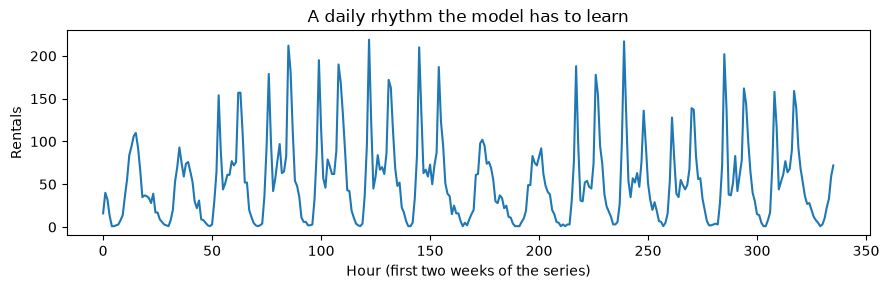
\includegraphics[width=.88\linewidth,height=5cm,keepaspectratio]{labs/visuals/08-notebook-reference.png}
\end{labvisual}
\begin{refoutput}
\begin{lstlisting}[style=utpterminal]
OLS test RMSE: 5829.38
OLS coefficients:    [3616.3 1978.4  519.2 9559.3]
Median GA coefficients: [3616.3 1978.4  519.2 9559.3]
\end{lstlisting}
\end{refoutput}

\textbf{What it means.} The GA's median test RMSE equals the OLS test RMSE to within rounding, and its coefficients match the OLS coefficients. Every seed drops onto the OLS line within a few dozen generations. The GA has \emph{found} the optimum; it has not \emph{beaten} it. For an unconstrained least-squares problem the closed-form solution is exact and far cheaper.
\end{labanswer}

\begin{labquestion}{6}{Run one sensitivity study}
Reduce the population from 100 to 40, repeat the ten seeds, and compare median test RMSE, its spread and runtime for both settings and OLS. Save \texttt{ga\_sensitivity\_pop40.csv} and \texttt{summary.csv}.
\end{labquestion}
\begin{labanswer}
\lstinputlisting[style=utppython,firstline=123,lastline=133]{all_experiments/lab08_genetic_algorithm_regression_worked.py}
\begin{refoutput}
\begin{lstlisting}[style=utpterminal]
       method  median_test_rmse  sd_test_rmse  median_runtime_s
0  GA pop=100         5829.3787        0.0019            0.0391
1   GA pop=40         5829.3819        0.0255            0.0176
2         OLS         5829.3785        0.0000               NaN
Saved: ['convergence.png', 'ga_10_runs.csv', 'ga_sensitivity_pop40.csv', 'split.csv', 'summary.csv']
\end{lstlisting}
\end{refoutput}

\textbf{What it means.} Forty chromosomes halve the runtime with the same median, and increase the seed-to-seed spread by more than ten times. On this easy problem both are fine. On a problem where a poor run is expensive, the spread is what you would be buying with those extra chromosomes.
\end{labanswer}

\begin{yourturn}
Add new cells at the end of the notebook. For every task, hold the split fixed, repeat over seeds 1--10, and report the median and standard deviation of test RMSE beside the OLS result. A helper saves typing:
\begin{lstlisting}[style=utppython]
def study(**settings):
    scores = [run_ga(seed, **settings)["test_rmse"] for seed in range(1, 11)]
    return round(np.median(scores), 2), round(np.std(scores, ddof=1), 4)
print(study(mutation_rate=0.0), study(mutation_rate=0.05), study(mutation_rate=0.5))
\end{lstlisting}
\begin{enumerate}
  \item \textbf{Mutation.} Try \texttt{mutation\_rate} 0, 0.05, 0.15 and 0.5, then \texttt{mutation\_scale} 0.01, 0.05, 0.25 and 1. What happens with no mutation at all, and why?
  \item \textbf{Budget.} Try \texttt{generations} 10, 20, 40 and 80. Where does extra budget stop paying?
  \item \textbf{Selection pressure.} Copy \texttt{run\_ga} and change the tournament size from 3 to 1, which means no selection at all. One result will look odd: the median test RMSE can fall \emph{below} the OLS value. Does that mean the GA has beaten least squares?
  \item \textbf{Write down one change} to the problem that would make a GA more appropriate than OLS, and what you would have to change in the fitness function or operators.
\end{enumerate}
\end{yourturn}

\begin{expectedfindings}
\begin{enumerate}
  \item With no mutation the median stays at about 6,534 with a spread of about 252: blending can only contract the population, so it collapses before reaching the optimum. Rates 0.05, 0.15 and 0.5 all reach about 5,829, with the tightest spread at 0.15. A scale of 0.01 is too timid (about 6,198); 0.05 and above reach the optimum.
  \item Median test RMSE is about 6,317, 5,952, 5,830 and 5,829.38. Almost nothing is gained after 80 generations, and the lab's 160 is a safe margin.
  \item With tournament size 1 the median is about 5,828.9 with a spread of about 11.5. It has not beaten anything. OLS minimises \emph{training} error, and it does so exactly. A run that has not converged can land closer to the test rows by chance, and the large spread is the giveaway. Its training RMSE is worse.
  \item Integer coefficients, a penalty on the number of non-zero coefficients, or a black-box cost all fit. Least squares no longer applies, so the fitness function changes, and integer genes would need new crossover and mutation.
\end{enumerate}
\end{expectedfindings}

\begin{troubleshoot}
\begin{description}
  \item[The GA never approaches OLS] Check the fitness sign (lower is better here) and that \texttt{X\_train} is the standardised matrix.
  \item[Results differ on every run] Pass the seed through to \texttt{np.random.default\_rng(seed)}. Do not use the global NumPy generator.
  \item[A shape error in \texttt{training\_mse}] Keep \texttt{individuals[:, [0]]} with the inner brackets, so that the intercept column broadcasts across the rows.
\end{description}
\end{troubleshoot}

\begin{verification}
\begin{itemize}
  \item The test GA finds $x\approx3$ for $f(x)=(x-3)^2$ before it is used on real data.
  \item The predictors are standardised with training statistics only (1,070 training and 268 test rows).
  \item Ten seeds are run, and \texttt{ga\_10\_runs.csv} records train RMSE, test RMSE and runtime for each.
  \item The GA's median test RMSE equals the least-squares test RMSE, and you can explain why it cannot beat it on training error.
  \item The population-40 sensitivity run is saved and its larger spread across seeds is explained.
\end{itemize}
\end{verification}

\begin{labdeliverable}
\begin{itemize}
  \item Restart the kernel and run all cells without errors.
  \item Submit the executed notebook, including your \emph{Your turn} cells, and the generated \texttt{results/lab08/} folder.
  \item Add a short conclusion: report the median and spread, explain why matching OLS is not beating it, and name one problem change that would make a GA more appropriate.
\end{itemize}
\end{labdeliverable}

